\section{Experimental Settings}

We evaluated the performance of the proposed method in relation to a large set of random sequences provided by state-of-the-art pseudo-random number generators.
In this section, we present the settings of the parameters that we use as a reference, the true random physical generators used to calculate the empirical distribution, and descriptive analysis of representative points in relation to the confidence regions.

\subsection{Parameters Settings and Dataset}

In the calculation of the ordinal symbol histogram, we employed the following factors in this study:
\begin{itemize}
\item Sequence length $T\in\mathcal T=\{10^3, \num[scientific-notation=true]{5 e4}\}$,
\item Embedding dimension $D\in\mathcal D=\{3, 4, 5, 6\}$,and
\item Time delay $\tau=\{1, 10, 30, 50\}$.
\end{itemize}

For the construction of the confidence regions presented, we use:
\begin{itemize}
    \item Set of $104596$ points in the $H \times C$ plane, referring to sequences of length $T = 1000$, for each combination of the factors $\mathcal T \times \mathcal D \times \mathcal{\tau}$, and
    \item  Another set of $2093$ points in the $H \times C$ plane, referring to sequences of length $T = 50000$, for each combination of factors $\mathcal T \times \mathcal D \times \mathcal{\tau}$.
\end{itemize}
Since the results involving the variation of the time delay parameter did not show a significant difference in repeated experiments, we don't consider it as a determinating factor during the execution of the algorithm.
On the other hand, we consider two determining variables during the generation of such sub-spaces: the embedding dimension and the length of the sequence.
%\todo[inline]{Justificar o porquê da ausência do tau nos experimentos}

The data generation and analyses were performed using the \texttt R platform \cite{Rmanual} v.~3.6.3.
We used the \texttt{ggplot2} library \cite{ggplot2Wickman} for generating the plots.

\subsection{True Random Numbers}

Random numbers are used in many fields, from gambling to criptography, aiming to guarantee a secure, realistic or unpredictable behavior. 
Pseudo randomic results can be achieved by software in a deterministic way. 
But, some applications need actual random numbers (despite the somewhat elusive nature of actual randomness).
Randomness can be observed in unpredictable real world phenomena like cathodic radiation or atmospheric noise.
%In this study we used two sources of real random numbers. 
%The first is based on vacuum states to generate random quantum numbers described by \citeauthor{RNGVacuumStates}~(\citeyear{RNGVacuumStates}), the second one is based on atmospheric noise captured by a cheap radio receiver presented at \url{www.random.org}.

In this study we used two sources of random numbers, here called true random, both from physical phenomena observation and measurement.
The first is based on vacuum states to generate random quantum numbers, the setup consists of an ordinary laser source to generate a local oscillator (LO), a half-wave plate, a polarizing beamsplitter (BPS), and two balanced detectors working together adding or subtracting the photocurrents results in a quadrature measurement of the LO or vacuum state. 
The probability distribution of the vacuum state is binned into $2^n$ equal parts (bins of same size), than, assigning a fixed bit combination of length \textit{n} to each sample point in a given bin \citeauthor{RNGVacuumStates}~(\citeyear{RNGVacuumStates}). 
The second one is based on atmospheric noise captured by a cheap radio receiver, started as a gambling engine, the randomness comes from an ordinary radio receiver that has no filter for static unwanted sounds caused by atmospheric noise, but perfect for random purposes, developed over a distributed setup with some radios located at different geographical locations sending random bits to a cloud server who process data and hosts random.org, the history, and some other information could be found at \cite{RandomOrg}.

%Deixei as URLs pois não tenho o .bib ...

%The colored $k$-noise mentioned in the previous section, also known as ``correlated noise'', is such that its power spectrum has shape $f^{-k}$.
%When $k=0$, we have white noise, i.e., independent deviates.
%The larger $k$ is, the more correlated the observations are.
\begin{comment}

\begin{figure}
    \centering
    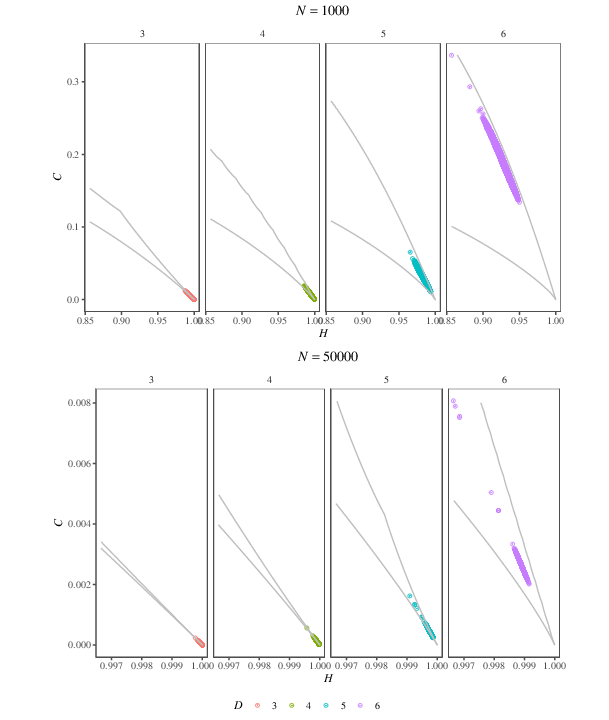
\includegraphics[width=\linewidth]{Figures/Points-PDF.png}
    \caption{White noise samples considered during the construction of the proposed confidence regions.}
    \label{fig:white-noise}
\end{figure}

\end{comment}